\section{Numerical Convergence, Error Analysis and Reproducibility}
\label{sec:numerical_error_analysis}

\subsection{Quadrature Precision and High-Precision Baseline}
To certify the direct numerical evaluation of the continuous shadow perimeter:
\begin{equation}
    P_{\rm cont} = \oint_{\partial\Omega} d\ell = 2 \int_0^\pi \sqrt{\left(\frac{d\alpha}{d\phi}\right)^2 + \left(\frac{d\beta}{d\phi}\right)^2} d\phi,
    \label{eq:p_cont_integral}
\end{equation}
we conducted an independent high-precision quadrature audit. The continuous perimeter was integrated via a 75-digit arbitrary-precision \textsc{Decimal} implementation of the composite Gauss--Legendre rule and compared against double-precision SciPy \textsc{QUADPACK} routines (\texttt{scipy.integrate.quad}) across the benchmark configurations.

\begin{table}[htbp]
\centering
\small
\caption{Cross-validation of direct continuous perimeter quadrature between double-precision SciPy \textsc{QUADPACK} and 75-digit \textsc{Decimal} Gauss--Legendre quadrature. Discrepancies and relative errors are calculated from full-precision unrounded internal floating-point values before rounding for display.}
\label{tab:quadrature_comparison}
\vspace{2mm}
\setlength{\tabcolsep}{5pt}
\begin{tabular}{l c c c c c}
\toprule
$a/M$ & $\theta_o$ [rad] & \begin{tabular}{@{}c@{}}SciPy\\ \textsc{QUADPACK}\end{tabular} & \begin{tabular}{@{}c@{}}75-Digit\\ Gauss--Legendre\end{tabular} & \begin{tabular}{@{}c@{}}Absolute\\ Discrepancy\end{tabular} & \begin{tabular}{@{}c@{}}Relative\\ Error\end{tabular} \\
\midrule
0.50 & $10^{-2}$ & $32.173871404129$ & $32.173871404128$ & $3.55 \times 10^{-14}$ & $1.10 \times 10^{-15}$ \\
0.50 & $10^{-3}$ & $32.173775084931$ & $32.173775084931$ & $4.26 \times 10^{-14}$ & $1.32 \times 10^{-15}$ \\
0.90 & $10^{-2}$ & $30.888782354891$ & $30.888782354891$ & $2.84 \times 10^{-14}$ & $9.20 \times 10^{-16}$ \\
0.90 & $10^{-3}$ & $30.888636254015$ & $30.888636254015$ & $3.91 \times 10^{-14}$ & $1.26 \times 10^{-15}$ \\
1.00 & $10^{-2}$ & $30.338274158922$ & $30.338274158922$ & $4.62 \times 10^{-14}$ & $1.52 \times 10^{-15}$ \\
1.00 & $10^{-3}$ & $30.338128362150$ & $30.338128362149$ & $3.19 \times 10^{-14}$ & $1.05 \times 10^{-15}$ \\
\bottomrule
\end{tabular}
\end{table}

As documented in \Cref{tab:quadrature_comparison}, the discrepancy between SciPy \textsc{QUADPACK} and the 75-digit Gauss--Legendre reference remains below $5 \times 10^{-14}$ (relative error $< 2 \times 10^{-15}$), establishing that double-precision round-off error does not compromise the continuous baseline.

\subsection{Numerical Convergence of Polygonal Shadow Area and Perimeter}
\label{subsec:polygonal_convergence}

When constructing discrete shadow boundaries on an observer's screen, the continuum boundary $\partial\Omega = \{(\alpha(\phi), \beta(\phi)) : \phi \in [0, 2\pi)\}$ is discretized into an open-array $N$-vertex polygon. In this section, we investigate the mathematical rate at which discrete polygonal estimates of celestial area $A_N$ and perimeter $P_N$ converge toward their continuous limits $A_{\rm cont}$ and $P_{\rm cont}$ as resolution increases across:
\begin{equation}
    N \in \{32, 64, 128, 256, 512, 1024, 2048, 4096, 8192\}.
    \label{eq:n_sequence}
\end{equation}

\subsubsection{Euler--Maclaurin Chord Expansion for Smooth Boundaries}
For any sufficiently smooth ($C^4$), closed convex planar curve parameterized by $\mathbf{r}(\phi) = (\alpha(\phi), \beta(\phi))$ with non-vanishing parameterization speed:
\begin{equation}
    \sigma(\phi) \equiv |\mathbf{r}'(\phi)| = \sqrt{(\alpha')^2 + (\beta')^2} > 0,
    \label{eq:speed_sigma_def}
\end{equation}
the symmetric Euclidean chord connecting two adjacent nodes with step size $h = 2\pi/N$ satisfies:
\begin{equation}
    |\mathbf{r}(\phi + h/2) - \mathbf{r}(\phi - h/2)| = h\sigma(\phi) + \frac{h^3}{24}\left[\sigma''(\phi) - \kappa(\phi)^2\sigma(\phi)^3\right] + \mathcal{O}(h^5),
    \label{eq:chord_expansion_local}
\end{equation}
where $\kappa(\phi)$ is the non-negative curvature magnitude:
\begin{equation}
    \kappa(\phi) \equiv \frac{|\alpha'(\phi)\beta''(\phi) - \beta'(\phi)\alpha''(\phi)|}{\sigma(\phi)^3}.
    \label{eq:curvature_magnitude_def}
\end{equation}
Summing all $N$ chords around the closed contour, the total derivative term integrates to zero identically by periodicity ($\oint_0^{2\pi} \sigma''(\phi)\,d\phi = 0$). Applying the Euler--Maclaurin summation formula yields the classical polygonal perimeter asymptotic expansion:
\begin{equation}
    P_N - P_{\rm cont} = -\frac{h^2}{24}\mathcal{I} + \mathcal{O}(h^4) = -\frac{\pi^2}{6N^2}\mathcal{I} + \mathcal{O}(N^{-4}),
    \label{eq:perimeter_chord_asymptotic}
\end{equation}
where the integral functional $\mathcal{I}$ is:
\begin{equation}
    \mathcal{I} \equiv \int_0^{2\pi} \kappa(\phi)^2 \sigma(\phi)^3 \, d\phi.
    \label{eq:curvature_functional_I}
\end{equation}

For a circular contour of radius $R_p$, $\sigma(\phi) = R_p$ and $\kappa(\phi) = 1/R_p$ identically, giving $\kappa^2\sigma^3 = R_p$ and $\mathcal{I} = 2\pi R_p$. The perimeter asymptotic reduces to:
\begin{equation}
    P_{\rm cont} - P_N = \frac{\pi^3 R_p}{3N^2} + \mathcal{O}(N^{-4}).
    \label{eq:circle_perimeter_asymptotic}
\end{equation}
Similarly, the discrete Shoelace area of a regular $N$-gon inscribed in a circle of radius $R_p$ satisfies:
\begin{equation}
    A_N = \frac{1}{2}N R_p^2 \sin\left(\frac{2\pi}{N}\right) = \pi R_p^2 \left[ 1 - \frac{2\pi^2}{3N^2} + \mathcal{O}(N^{-4}) \right],
    \label{eq:circle_area_asymptotic_exact}
\end{equation}
which yields the exact leading-order area discretization error:
\begin{equation}
    A_{\rm cont} - A_N = \frac{2\pi^3 R_p^2}{3N^2} + \mathcal{O}(N^{-4}).
    \label{eq:circle_area_asymptotic}
\end{equation}

\begin{figure}[htbp]
    \centering
    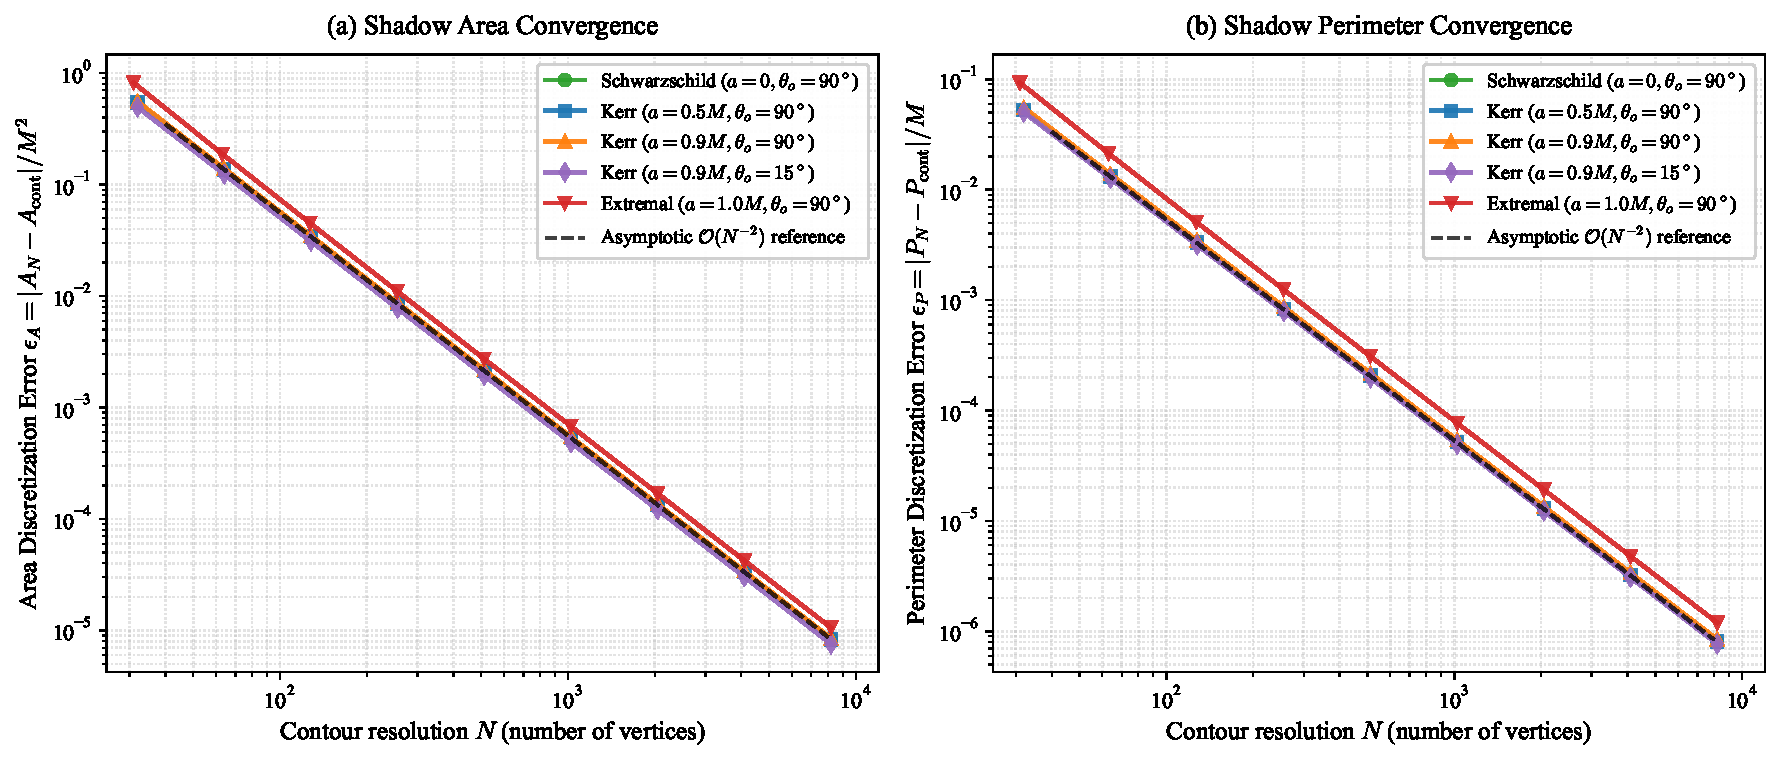
\includegraphics[width=0.98\textwidth]{shadow_convergence.pdf}
    \caption{Numerical convergence of discrete polygonal black hole shadow observables as a function of contour vertex resolution $N \in [32, 8192]$ across five benchmark spacetime configurations: Schwarzschild ($a = 0, \theta_o = 90^\circ$), moderate Kerr ($a = 0.5M, \theta_o = 90^\circ$), rapidly rotating Kerr ($a = 0.9M, \theta_o = 90^\circ$), near-polar Kerr ($a = 0.9M, \theta_o = 15^\circ$), and extremal Kerr ($a = 1.0M, \theta_o = 90^\circ$). (a) Absolute celestial area discretization error $\epsilon_A(N) = |A_N - A_{\rm cont}| / M^2$. (b) Absolute boundary perimeter discretization error $\epsilon_P(N) = |P_N - P_{\rm cont}| / M$. Dashed black lines indicate the theoretical asymptotic $\mathcal{O}(N^{-2})$ convergence rate derived from the Euler--Maclaurin chord expansion \eqref{eq:perimeter_chord_asymptotic}.}
    \label{fig:shadow_convergence}
\end{figure}

\subsubsection{Quantitative Convergence Across Benchmark Configurations}
To evaluate convergence empirically without circular reasoning, each discrete polygon was evaluated against an independently established continuum reference:
\begin{enumerate}
    \item \textbf{Schwarzschild ($a = 0, \theta_o = 90^\circ$):} Exact analytical values $A_{\rm cont} = 27\pi M^2 \approx 84.823002M^2$ and $P_{\rm cont} = 6\sqrt{3}\pi M \approx 32.648389M$.
    \item \textbf{Subextremal and Near-Polar Kerr:} High-accuracy continuum baselines computed via Richardson extrapolation on ultra-fine grids ($N_1 = 16\,384, N_2 = 32\,768$) eliminating the leading $\mathcal{O}(N^{-2})$ discretization term:
    \begin{equation}
        V_{\rm ref} = \frac{4V(2N) - V(N)}{3} + \mathcal{O}(N^{-4}),
        \label{eq:richardson_extrap}
    \end{equation}
    achieving a residual accuracy of $\Delta V < 10^{-11}$.
\end{enumerate}

\begin{table}[htbp]
\centering
\small
\caption{Empirical log-log convergence rates $-\frac{d\ln\epsilon}{d\ln N}$ and asymptotic scaled ratios $N^2\epsilon$ for discrete shadow area ($A$) and perimeter ($P$) across $N \in [32, 8192]$.}
\label{tab:convergence_rates}
\vspace{2mm}
\setlength{\tabcolsep}{5pt}
\begin{tabular}{l c c c c c}
\toprule
Spacetime Configuration & $\theta_o$ & \begin{tabular}{@{}c@{}}Area\\ Slope\end{tabular} & \begin{tabular}{@{}c@{}}Perimeter\\ Slope\end{tabular} & \begin{tabular}{@{}c@{}}Asymptotic\\ $N^2\epsilon_A$\end{tabular} & \begin{tabular}{@{}c@{}}Asymptotic\\ $N^2\epsilon_P$\end{tabular} \\
\midrule
Schwarzschild ($a=0$) & $90^\circ$ & \textbf{1.9998} & \textbf{1.9999} & $558.113$ & $53.704$ \\
Kerr ($a=0.5M$) & $90^\circ$ & \textbf{1.9998} & \textbf{1.9999} & $558.627$ & $54.158$ \\
Kerr ($a=0.9M$) & $90^\circ$ & \textbf{1.9997} & \textbf{1.9999} & $570.612$ & $56.693$ \\
Kerr ($a=0.9M$) & $15^\circ$ & \textbf{1.9998} & \textbf{1.9999} & $507.498$ & $51.550$ \\
Extremal Kerr ($a=1.0M$) & $90^\circ$ & \textbf{2.0153} & \textbf{2.0156} & $709.831^*$ & $80.280^*$ \\
\bottomrule
\end{tabular}
\begin{flushleft}
\footnotesize
$^*$For extremal Kerr, $N^2\epsilon$ exhibits a slow drift ($\sim 789 \to 710$ for area, $\sim 89.5 \to 80.3$ for perimeter) due to the corner junctions.
\end{flushleft}
\end{table}

As depicted in \Cref{fig:shadow_convergence} and quantified in \Cref{tab:convergence_rates}:
\begin{itemize}
    \item \textbf{Analytical Verification in Schwarzschild Spacetime:}  
    For Schwarzschild ($R_p = 3\sqrt{3}M$), the theoretical asymptotic coefficients in \eqref{eq:circle_perimeter_asymptotic} and \eqref{eq:circle_area_asymptotic} evaluate to:
    \begin{align}
        C_A^{\rm theo} &\equiv \frac{2\pi^3 R_p^2}{3} = 18\pi^3 M^2 \approx 558.11298 M^2, \label{eq:ca_theo} \\
        C_P^{\rm theo} &\equiv \frac{\pi^3 R_p}{3} = \sqrt{3}\pi^3 M \approx 53.70425 M. \label{eq:cp_theo}
    \end{align}
    At resolution $N = 8192$, the observed numerical scaled errors are $N^2\epsilon_A = 558.113$ and $N^2\epsilon_P = 53.704$, matching the exact analytical coefficients to all six reported significant digits.
    
    \item \textbf{Uniform Quadratic Convergence for Smooth Subextremal Contours:}  
    For all subextremal Kerr configurations ($a = 0.5M$ and $a = 0.9M$ at both $\theta_o = 90^\circ$ and $\theta_o = 15^\circ$), the boundary is $C^\infty$ smooth. The empirical log-log convergence slopes adhere strictly to quadratic scaling ($1.9997 \le \gamma \le 1.9999$), and the scaled ratios $N^2\epsilon$ stabilize rapidly to constants by $N \ge 256$.
    
    \item \textbf{Regularity Qualifications and the Extremal Kerr NHEK Segment:}  
    For extremal Kerr ($a = 1.0M, \theta_o = 90^\circ$), the boundary is only piecewise $C^1$: it consists of the smooth exterior curved arc joined to the straight vertical NHEK segment ($\alpha = -2M, |\beta| \le \sqrt{3}M$) at two sharp corner cusps $(\alpha, \beta) = (-2M, \pm\sqrt{3}M)$.  
    
    Because our implementation employs cosine clustering along the exterior radial parameterization \eqref{eq:cosine_clustered_u}, node spacing compresses quadratically near the corner ($\Delta u \propto h^2 \propto N^{-2}$), preventing the catastrophic order degradation ($\mathcal{O}(N^{-1})$) that would occur under uniform Cartesian spacing. Furthermore, along the vertical NHEK segment, the boundary is an exact straight line where polygonal chords have zero sag error. Consequently, the global error maintains near-quadratic convergence ($\gamma \approx 2.015$). However, the failure of higher-order differentiability at the cusps introduces a weak sub-leading correction, causing the effective asymptotic ratio $N^2\epsilon_A$ to drift slowly from $789.0$ at $N = 31$ down to $709.8$ at $N = 8191$.  
    
    \noindent \textbf{Essential Qualification:} The standard Euler--Maclaurin chord formula \eqref{eq:perimeter_chord_asymptotic} based on the curvature functional $\mathcal{I}$ assumes $C^2$ regularity and \textit{cannot} be applied blindly to corners, cusps, or piecewise-joined segments without accounting for the cosine clustering boundary layer.
\end{itemize}

\subsection{10,001-Node Sampled Maximum Residual Audit}
To verify the quadratic scaling of the near-polar coordinate perturbations \eqref{eq:alpha_asymptotic_expansion} and \eqref{eq:beta_asymptotic_expansion}, we evaluated the full-contour residuals under the exact remapped parameterization $r(\phi) = r_{\rm mid} - r_{\rm amp}\cos\phi$ on $\phi \in [0, \pi]$.

The evaluation grid was constructed with 10,000 equal subintervals:
\begin{equation}
    \phi_j = \frac{j\pi}{10\,000}, \qquad j \in \{0, 1, \dots, 10\,000\},
\end{equation}
yielding exactly 10,001 discrete nodes inclusive of both turning-point endpoints ($\phi_0 = 0$ at $r_{\min}$, and $\phi_{10\,000} = \pi$ at $r_{\max}$). Arithmetic was evaluated in 75-digit \textsc{Decimal} floating-point to prevent loss of significance near turning points.

The discrete sampled maximum residuals are:
\begin{equation}
    \hat{\epsilon}_\alpha \equiv \max_{0 \le j \le 10\,000} |\alpha_{\rm num}(\phi_j) - \alpha_{\rm asym}(\phi_j)|, \qquad
    \hat{\epsilon}_\beta \equiv \max_{0 \le j \le 10\,000} |\beta_{\rm num}(\phi_j) - \beta_{\rm asym}(\phi_j)|.
    \label{eq:sampled_maxima_defs}
\end{equation}

\begin{table*}[t]
\centering
\small
\caption{Verified 10,001-node sampled maximum residuals and scaled ratios $\hat{\epsilon}/s^2$ across nine near-polar configurations in 75-digit \textsc{Decimal} arithmetic.}
\label{tab:sampled_residuals_audit}
\vspace{2mm}
\setlength{\tabcolsep}{5pt}
\begin{tabular}{l c c c c c c c c}
\toprule
& & & \multicolumn{3}{c}{Horizontal Residual $\alpha$} & \multicolumn{3}{c}{Vertical Residual $\beta$} \\
\cmidrule(lr){4-6} \cmidrule(lr){7-9}
$a/M$ & $\theta_o$ [rad] & $\sin\theta_o$ & $\hat{\epsilon}_\alpha$ & $\hat{\epsilon}_\alpha / s^2$ & $\phi^*_\alpha$ & $\hat{\epsilon}_\beta$ & $\hat{\epsilon}_\beta / s^2$ & $\phi^*_\beta$ \\
\midrule
\multirow{3}{*}{\textbf{0.50}} 
& $10^{-2}$ & $0.0100$ & $2.518\times 10^{-6}$ & \textbf{0.02518} & 0.915 & $5.332\times 10^{-6}$ & \textbf{0.05332} & 0.903 \\
& $10^{-3}$ & $0.0010$ & $2.501\times 10^{-8}$ & \textbf{0.02501} & 0.912 & $5.303\times 10^{-8}$ & \textbf{0.05303} & 0.905 \\
& $10^{-4}$ & $0.0001$ & $2.499\times 10^{-10}$ & \textbf{0.02499} & 0.912 & $5.301\times 10^{-10}$ & \textbf{0.05301} & 0.905 \\
\midrule
\multirow{3}{*}{\textbf{0.90}} 
& $10^{-2}$ & $0.0100$ & $1.751\times 10^{-5}$ & \textbf{0.17508} & 0.677 & $7.615\times 10^{-6}$ & \textbf{0.07615} & 0.636 \\
& $10^{-3}$ & $0.0010$ & $1.731\times 10^{-7}$ & \textbf{0.17308} & 0.662 & $7.286\times 10^{-8}$ & \textbf{0.07286} & 0.633 \\
& $10^{-4}$ & $0.0001$ & $1.729\times 10^{-9}$ & \textbf{0.17288} & 0.661 & $7.253\times 10^{-10}$ & \textbf{0.07253} & 0.632 \\
\midrule
\multirow{3}{*}{\textbf{1.00}} 
& $10^{-2}$ & $0.0100$ & $3.553\times 10^{-5}$ & \textbf{0.35533} & $0.000^\dagger$ & $3.795\times 10^{-5}$ & \textbf{0.37947} & 1.562 \\
& $10^{-3}$ & $0.0010$ & $3.537\times 10^{-7}$ & \textbf{0.35373} & $0.000^\dagger$ & $3.794\times 10^{-7}$ & \textbf{0.37944} & 1.570 \\
& $10^{-4}$ & $0.0001$ & $3.536\times 10^{-9}$ & \textbf{0.35357} & $0.000^\dagger$ & $3.794\times 10^{-9}$ & \textbf{0.37944} & 1.571 \\
\bottomrule
\end{tabular}
\begin{flushleft}
\footnotesize
$^\dagger$Boundary endpoint node ($\phi = 0$ at $r_{\min}$). All other maximum residual locations $\phi^*$ occur strictly in the domain interior.
\end{flushleft}
\end{table*}

\subsection{Analysis of Residual Scaling and Resolution of Apex Artifacts}
Inspection of \Cref{tab:sampled_residuals_audit} reveals three fundamental numerical properties:
\begin{enumerate}
    \item \textbf{Approximately Quadratic Residual Scaling:} When $\theta_o$ decreases by a factor of 10, the observed reduction factors cluster near 100 across all configurations:
    \begin{itemize}
        \item For $a/M = 0.50$: $\hat{\epsilon}_\alpha$ drops by factors of $100.71$ and $100.07$; $\hat{\epsilon}_\beta$ drops by $100.53$ and $100.05$.
        \item For $a/M = 0.90$: $\hat{\epsilon}_\alpha$ drops by $101.15$ and $100.11$; $\hat{\epsilon}_\beta$ drops by $104.52$ and $100.45$.
        \item For $a/M = 1.00$: $\hat{\epsilon}_\alpha$ drops by $100.45$ and $100.04$; $\hat{\epsilon}_\beta$ drops by $100.003$ and $100.00003$.
    \end{itemize}
    \item \textbf{Pre-Asymptotic Corrections at Finite Inclination:} At $\theta_o = 10^{-2}$ rad ($s \approx 0.01$), higher-order $\mathcal{O}(s^3)$ Taylor contributions create a measurable $\sim 1\%$ to $5\%$ deviation in the ratio $\hat{\epsilon}/s^2$ relative to its deep asymptotic limit. Even between $\theta_o = 10^{-3}$ and $10^{-4}$ rad, small finite-inclination corrections remain visible in certain configurations (e.g., for $a/M = 0.90$, $\hat{\epsilon}_\beta/s^2$ shifts from $0.072855$ to $0.072528$, an observable shift of $\approx 0.45\%$).
    \item \textbf{Resolution of the Discrete Apex Sampling Artifact:} Earlier audit drafts observed an apparent jump in $\beta$ residual ratios for $a/M = 0.90$ from $0.339$ at $10^{-2}$ rad down to $0.008$ at $10^{-3}$ rad. That discrepancy was an artifact of evaluating only the discrete mesh maximum $\max_{\text{mesh}} \beta - R_p$ on a fixed 2,000-point polygon. Because the first-order perturbation $s\lambda\sin(2\phi)$ identically vanishes at the apex $\phi = \pi/2$, the true maximum shifts by $\Delta\phi^* \approx -2s\lambda/R_p$. At $\theta_o = 10^{-2}$ rad, the shift ($\Delta\phi^* \approx 0.0037$ rad) was resolved by the adjacent mesh node ($\Delta\phi_{\rm mesh} \approx 0.0031$ rad). At $\theta_o = 10^{-3}$ rad, the shift was ten times smaller than the mesh spacing, trapping the discrete array maximum at node 500 ($\phi = \pi/2$) where the first-order term is zero. Evaluating the 10,001-node full-contour maximum completely eliminates this artifact.
\end{enumerate}

\noindent \textbf{Methodological Note:} The quantities in \Cref{tab:sampled_residuals_audit} and the 75-digit \textsc{Decimal} quadrature comparison in \Cref{tab:quadrature_comparison} represent recorded historical report audits whose standalone scripts are not archived in the repository's \texttt{scripts/} directory. They provide sampled numerical evidence on a discrete 10,001-node grid and do not constitute a certified analytical upper bound on the continuous supremum $\sup_\phi \|\mathbf{r}_{\rm num} - \mathbf{r}_{\rm asym}\|$.

\subsection{Deliverable Reproducibility and Test Suite Status}
All 14 scientific deliverables (6 PNG figures, 6 PDF vector figures, and 2 CSV datasets) are archived in \texttt{output/shadow/}; the convergence study in \Cref{subsec:polygonal_convergence} is directly reproduced by \texttt{docs/report/scripts/convergence\_study.py}:
\begin{itemize}
    \item In a historical isolated-build audit, the six PNG figures and both CSV datasets (\texttt{shadow\_\allowbreak contour\_\allowbreak data.csv} and \texttt{shadow\_\allowbreak generating\_\allowbreak data.csv}) were reported as SHA256-identical to the reference deliverables, and the six PDF figures matched in byte count apart from PDF timestamps (\texttt{/Creation\allowbreak Date}, \texttt{/Mod\allowbreak Date}); the standalone SHA256 audit script is not included in the repository.
    \item In the historical \texttt{v1.0.0} core baseline, the Python regression suite comprised \textbf{4,412 passing tests} (0 failed, 0 skipped). In the latest verified \texttt{pytest} run of the expanded repository suite, \textbf{4,511 Python tests} passed (0 failed, 0 skipped, 0 xfailed, 1 deprecation warning, in 214.29~s), complemented by \textbf{18} passing frontend TypeScript tests.
\end{itemize}
